% ----------------------------------------------------------------
% AMS-LaTeX Paper ************************************************
% **** -----------------------------------------------------------
%\documentclass{article}

\documentclass[letterpaper, 10 pt, conference]{IEEEconf}

%\usepackage{graphicx}
%\usepackage{algorithm}
\usepackage{amsmath}
\usepackage{siunitx}
\usepackage{verbatim}
\usepackage[normalem]{ulem}
\usepackage{graphicx}
\graphicspath{{images/}}
% ----------------------------------------------------------------
\vfuzz2pt % Don't report over-full v-boxes if over-edge is small
\hfuzz2pt % Don't report over-full h-boxes if over-edge is small
% THEOREMS -------------------------------------------------------
\newtheorem{thm}{Theorem}[section]
\newtheorem{cor}[thm]{Corollary}
\newtheorem{lem}[thm]{Lemma}
\newtheorem{prop}[thm]{Proposition}

\newtheorem{defn}[thm]{Definition}

\newtheorem{rem}[thm]{Remark}

% MATH -----------------------------------------------------------
\newcommand{\norm}[1]{\left\Vert#1\right\Vert}
\newcommand{\card}[1]{\left|#1\right|}
\newcommand{\abs}[1]{\left\vert#1\right\vert}
\newcommand{\set}[1]{\left\{#1\right\}}
\newcommand{\Real}{\mathbb R}
\newcommand{\eps}{\varepsilon}
\newcommand{\To}{\longrightarrow}
\newcommand{\BX}{\mathbf{B}(X)}
\newcommand{\A}{\mathcal{A}}
% ----------------------------------------------------------------
\begin{document}

\title{\LARGE\bfseries Parallelization of the Needleman-Wunsch Algorithm}

\author{
	Klasing, Blake\\
	University of Central Florida \\
	Orlando, FL \\
	\texttt{BKlasing@knights.ucf.edu}
	\and
	Gramajo, Stacy\\
	University of Central Florida \\
	Orlando, FL \\
	\texttt{SGramajo@knights.ucf.edu} \\
	}
\maketitle
% ----------------------------------------------------------------
\section{Abstract}

In Bioinformatics, one of the well-known problem is understanding evolutionary relationships through sequence alignments that can be found in a number set of data: protein, DNA, RNA, or genes. A fundamental method used for global sequence alignment is Needleman-Wunsch algorithm. It solves the problem of finding the optimal alignment among two sequences, based on a simple scoring system. We propose to examine this algorithm and implement a parallelized program that can decrease the execution time for analyzing two sequences without sacrificing correctness and time complexity.


\section{Introduction}

The Needleman-Wunsch(NW) algorithm is global sequence alignment method that exemplifies the relationship between sequences using a scoring system. Using a dynamic programming approach, there are two parts to the algorithm in order to retrieve the optimal score: creating a matrix and traceback. The traceback method is somewhat trivial that can be accomplished in linear time. However, the creation of the scoring matrix poses a more complex problem that we will be focusing on. 

Overall, the NW algorithm achieves a $O(n\cdot m)$ time complexity and $O(n\cdot m)$ space complexity, where $n$ and $m$ are the lengths of the input sequences to be aligned. Although this is not an issue if the sequences are small, as they increase, the size of the scoring matrix as well as computing it grows in a quadratic fashion. For huge datasets that are the norm within the computational biology field, this poses an issue. For this reason, speeding up this algorithm can have great affects within the bioinformatics community, if not at least provide some insight into how to parallelize such an algorithm. 

We propose to parallelize the method that computes the scoring matrix within the NW algorithm in order to improve the overall execution time. Our main goal is to achieve reasonable speedup versus the original NW algorithm by utilizing current consumer grade multicore processing architectures. 

\section{Related Work}
The Needleman-Wunsch algorithm is widely known for solving this fundamental biology problem of global RNA sequence alignment. An algorithm proposed by Temple F. Smith and Michael S. Waterman is also very well known for solving a very similar problem, local RNA sequence alignment \cite{smith_waterman_1981}. Both of these algorithms solve the problem of optimal RNA alignment by dynamic programming, reaching the same time complexity. There are many other implementations and concepts of solving the problem of non-structured optimal RNA alignment, but we will focus on the NW dynamic programming solution.

Some parallelized implementations of NW take advantage of the hardware being used to not only speed up the original non-parallelized algorithm, but also push this hardware to its limits in order to squeeze as much computation as possible out of it with a parallelized algorithm. A group of researchers at the University of Delaware create a highly parallelized implementation based on fine grain multithreaded execution and architecture model \cite{martins_2001}. 
 
The majority of research around parallelizing the NW algorithm focuses on speeding up the calculation of the scoring matrix, which is where most of the computation takes place. However, some researchers focus on both the method of creating the scoring matrix, as well as the backtracking method \cite{seguel_2011}. Researchers at the University of Puerto Rico at Mayaguez bring a more complete approach of parallelizing the NW algorithm by offering a parallel implementation of the backtracking method, in addition to the scoring matrix method. This group of researchers take advantage of properties of symmetry between the matrix $D$ and $D'$, where $D$ is a matrix based on the original sequences being aligned, and $D'$ is a matrix based on the same sequences in reverse order.

Other approaches include dividing the input sequences into several smaller sequences, calculating the matrices, backtracking to find the optimal score, and combining the results from each set of sequence alignments. This method is based on finding local optimal sequence alignment. This implies that it is not guaranteed to find the optimal global sequence alignment score. However, it may provide insight into possible solutions to parallelizing this global optima algorithm \cite{zhang_2004}.  

\section{Background}

\subsection{Needleman-Wunsch}

To compute the NW, the algorithm needs two sequences as the input. Assuming in this case that sequence 1 is m and sequence 2 is n. Using the sequences, a table is created where the number of rows equal to length of m+1 and the number of columns equal to the length of n+1. After the creation of the matrix S, the first row and column in precomputed. Then the matrix takes each of the remaining cells in the matrix and computes the maximum of three equations: 


\begin{equation}
	S(i, j) = max 
	\begin{cases}
		S(i-1, j-1) + c(i, j)\\
		S(i-1, j) + c(i, -)\\
		S(i, j-1) + c(-, j)\\
	\end{cases}
\end{equation}

Once S has been filled, the final score is taken by the last item that was inputted. In order to print out the string containing gaps, mismatches, or matches, NW uses S to trace back starting at S [m+1, n+1].

The scoring system that is used to determine the overall score consists of three types of variables used: Gap, Mismatch, and Match. Gap is represented as the ‘-‘ character symbol that will appear in either/both of the sequences as the output solution. Match is the number added in the score if the characters of index i equal each other. Mismatch is usually a negative value that decrease the final score. 

\subsection{Multiprocessor Programming Concepts}
In both the lock-based and lock-free implementation, it uses an unbounded pool as one of its architecture design. A bounded or unbounded item determines if the structure is limited to a specific capacity. If the object is unbounded, then it is not confined to a size; whereas, bounded is visa-versa. A pool is an object that contains methods where producer threads is able to store items and consumer threads are able to retrieve items to work on. 

The lock-based method will contain a few mutexes. Mutexes are locks used to ensure mutual exclusion on critical sections. The lock-free does not use synchronization primitives, such as the mutex. It is a program that must be thread-safe when accessing a shared data. When constructing a lock-free program, primitives like the CAS (compare-and-swap) is used. The CAS is a type of instruction that has three parameters: the address of object x, value it is expected e, and value that it needs to change to v. When it is executed, CAS checks if x is equal to e. If true, then the value is updated to v and returns true; otherwise, x is not altered and returns false. 

\section{Implementation Overview}
\subsection{Lock Based Implementation 1}
The first implementation of a parallel NW algorithm makes use of a single lock and a pool, implemented as an array(vector). Before the algorithm starts spinning up threads to do work, the first row/column of the scoring matrix is computed. These computations are somewhat trivial and are only based on the previous single calculation. The main idea of this implementation is as follows: The first thread begins to calculate the first cell. When it is finished, the thread adds two items into the pool where other threads can retrieve and start computing its score. This cycle continues until the matrix has been complete.
The lock in this implementation allows us to ensure no issues arise when accessing the pool. For instance, if a thread takes an element from the pool to work on, it may be possible that another thread attempts to access the same element. We must lock each time we enqueue an element into the pool, as well as whenever we check or dequeue an element. 
This implementation is a somewhat coarse grain locking implementation, where this single lock becomes a bottleneck, especially with the addition of threads. This means that this implementation's performance will suffer greatly as it is scaled up with multiple CPUs(threads). As more CPUs are performing operations in this implementation, they must all be stopped for one single thread whether it is enqueueing, dequeueing, or simply checking the pool. 
\subsection{Lock Based Implementation 2}
In this lock based implementation, we use the same approach of how to solve the problem. However, we use two different locks, one for enqueueing and one for dequeueing from the pool. In this implementation, the pool is implemented as a linked list, in which we use head and tail pointers. This allows us to access the pool with less constraint. As long as the pool is not empty, threads will experience much less time waiting. This means we can asynchronously dequeue and enqueue while there is something in the pool. 
This is an attempt to speed up our first lock based implementation and provide a finer grain locking protocol. 
\subsection{Lock Free Implementation}



\section{Experimental Results}


\begin{figure*}
\centering
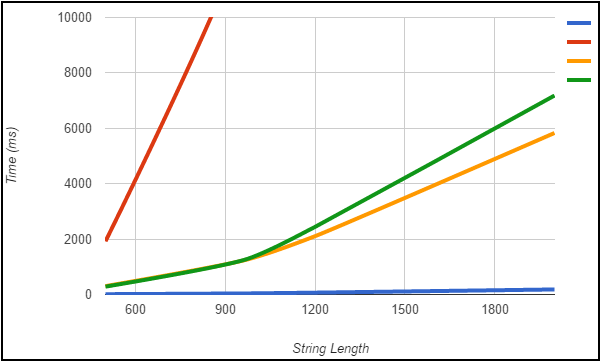
\includegraphics[scale=0.6]{sequential_vs_parallel}
\caption{Sequential vs Parallel Implementations}
\medskip
\small
Red: Lock Based \#1\\ Green: Lock Based \#2\\ Orange: Lock Free\\ Blue: Sequential    
\end{figure*}




\useunder{\uline}{\ul}{}
\begin{table*}[t]
	\centering
	\caption{}
	\label{my-label}
	\begin{tabular}{ccccc}
		{\ul Sequence Length}                                                                     & \begin{tabular}[c]{@{}c@{}}Sequential\\ (\end{tabular} & \begin{tabular}[c]{@{}c@{}}Lock \#1\\ (2 thread)\end{tabular} & \begin{tabular}[c]{@{}c@{}}Lock \#2\\ (2 thread)\end{tabular} & \begin{tabular}[c]{@{}c@{}}Lock Free\\ (2 thread)\end{tabular} \\ \hline
		\multicolumn{1}{|c|}{\begin{tabular}[c]{@{}c@{}}500\\ (Bison - Hamster)\end{tabular}}     & \multicolumn{1}{c|}{0.011716}                          & \multicolumn{1}{c|}{1.92007}                                  & \multicolumn{1}{c|}{0.302479}                                 & \multicolumn{1}{c|}{0.283637}                                  \\ \hline
		\multicolumn{1}{|c|}{\begin{tabular}[c]{@{}c@{}}974\\ (Rabbit - Polar Bear)\end{tabular}} & \multicolumn{1}{c|}{0.038957}                          & \multicolumn{1}{c|}{13.3043}                                  & \multicolumn{1}{c|}{1.26447}                                  & \multicolumn{1}{c|}{1.28418}                                   \\ \hline
		\multicolumn{1}{|c|}{\begin{tabular}[c]{@{}c@{}}1200\\ (Fish - Dolphin)\end{tabular}}     & \multicolumn{1}{c|}{0.066464}                          & \multicolumn{1}{c|}{23.9059}                                  & \multicolumn{1}{c|}{2.10464}                                  & \multicolumn{1}{c|}{2.44018}                                   \\ \hline
		\multicolumn{1}{|c|}{\begin{tabular}[c]{@{}c@{}}2000\\ (Goat - Giraffe)\end{tabular}}     & \multicolumn{1}{c|}{0.18204}                           & \multicolumn{1}{c|}{107.214}                                  & \multicolumn{1}{c|}{5.8305}                                   & \multicolumn{1}{c|}{7.18229}                                   \\ \hline
	\end{tabular}
\end{table*}

\section{Conclusion}
-TBD-

\section{Appendix}
\subsection{Challenges}
\begin{itemize}
	\item
	Lock based implementation
	\item
	Achieving speedup against the original NW algorithm
	\item 
	Achieving speedup comparable to other parallel implementations of sequence alignment algorithms
	\item
	using pools effectively to avoid ABA
	\item 
	acquiring implementations of related work that will compared against our algorithm. 
\end{itemize}

\subsection{Completed Tasks}
\begin{itemize}
	\item
	Implementation of sequential Needleman-Wunsch algorithm
	\item
	Abstract/Introduction/Related Work/Background complete within report
	\item
	Dataset acquired to test our algorithms
\end{itemize}


\subsection{Remaining Tasks}
\begin{itemize}
	\item
	Complete parallel implementation of algorithm
	\item
	Create testing suite to ensure results are correct
	\item
	Indentify concurrency validation software to use
	\item
	Gathering results for comparing with our algorithm
	\item
	Complete report
\end{itemize}


\bibliography{references}
\bibliographystyle{plain}

\begin{comment}

Martins, W. S., et al. "A multithreaded parallel implementation of a dynamic programming algorithm for sequence comparison." Pacific Symposium on Biocomputing. Vol. 6. 2001.
Url: http://wwwmayr.in.tum.de/lehre/2007SS/cb/reading/Martins01.pdf

2. Seguel, Jaime, and Carlos Torres. "Paralellization of Needleman-Wunsch String Alignment Method." (2011): 239-244.
Url: http://www.worldcomp-proceedings.com/proc/p2011/BIC5034.pdf

3. Devi, S. Nirmala, and S. P. Rajagopalan. "A modified dynamic parallel algorithm for sequence alignment in biosequences." International Journal of Computer Applications 60.18 (2012).
Url: http://citeseerx.ist.psu.edu/viewdoc/download?doi=10.1.1.303.3050&rep=rep1&type=pdf

4. de la Torre, Luis, and Jaime Seguel. "A Parallel Needleman-Wunsch-Hirschberg Bio-sequence Alignment Algorithm." CSC. 2010.
Url: https://www.researchgate.net/publication/221142998_A_Parallel_Needleman_-_Wunsch_-_Hirschberg_Bio-sequence_Alignment_Algorithm 

5. 
Fa, Z; Xiang-Zhen, Q; Zhi-Yong, L. A parallel Smith-Waterman algorithm based on divide and conquer. Proceedings Fifth International Conference on Algorithms & Architectures for Parallel Processing, 2002. 162, Jan. 2002.


6. Smith, Temple F., and Michael S. Waterman. "Identification of Common Molecular Subsequences." Journal of Molecular Biology 147.1 (1981): 195-97. Web.
http://dornsife.usc.edu/assets/sites/516/docs/papers/msw_papers/msw-042.pdf 

---- Book Reference
Herlihy, Maurice, and Nir Shavit. The Art of Multiprocessor Programming. Amsterdam: Elsevier/Morgan Kaufmann, 2008. Print.

-- understanding the NW problem reference

"Needleman–Wunsch Algorithm." Wikipedia. Wikimedia Foundation, n.d. Web.
\end{comment}

 % ----------------------------------------------------------------
\end{document}
% ----------------------------------------------------------------
